\documentclass{beamer}
\usetheme{metropolis}
\usepackage{graphicx}
\usepackage{amsmath}
\usepackage{tcolorbox}

\def\rcurs{{\mbox{$\resizebox{.16in}{.08in}{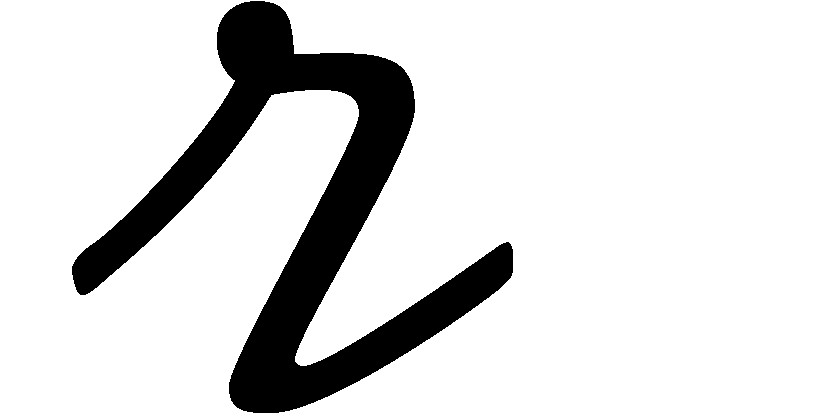
\includegraphics{ScriptR}}$}}}
\def\brcurs{{\mbox{$\resizebox{.16in}{.08in}{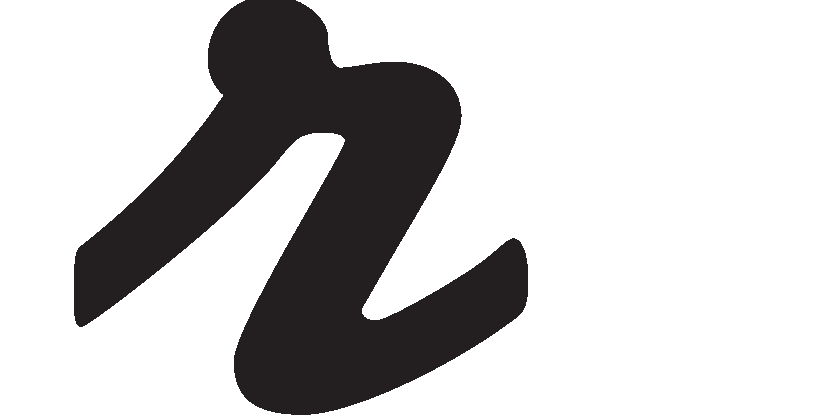
\includegraphics{BoldR}}$}}}
\def\hrcurs{{\mbox{$\hat \brcurs$}}}

\title{Electromagnetc Theory: PHYS330}
\author{Jordan Hanson}
\institute{Whittier College Department of Physics and Astronomy}

\begin{document}
\maketitle

\section{Summary}

\begin{frame}{Week 2 Summary}
\begin{enumerate}
\item Homework discussions
\begin{itemize}
\item Proofs!  Glorious proofs.
\item Exercises with \textit{checking} fundamental theorems
\end{itemize}
\item Electrostatics and Coulomb forces
\begin{itemize}
\item Charge distributions, superposition, and the Coulomb force
\item A note about the \textit{far-field}
\item Setting up integrals, taking limits, checking units
\item The divergence of electric fields
\item The curl of electric fields
\end{itemize}
\item Electric Potential
\begin{itemize}
\item Definitions, fundamental theorem for gradients
\item Reference points
\item Laplace equation ...
\end{itemize}
\item Work, energy, and conductors
\end{enumerate}
\end{frame}

\section{Homework}

\begin{frame}{Homework, Week 2}
Unlike last week, these exercises come from \textit{within} the chapter.  Ideally, you should look at all of the problems within the chapter as you study.
\begin{itemize}
\item Exercise 2.5
\item Exercise 2.6
\item Exercise 2.9
\item Exercise 2.12
\item Exercsie 2.16
\item Exercise 2.18
\item Exercise 2.25
\item Exercise 2.29
\end{itemize}
\end{frame}

\section{Charge distributions, Superposition, and the Coulomb Force}

\begin{frame}{Charge distributions, Superposition, and the Coulomb Force}
\begin{figure}
\centering
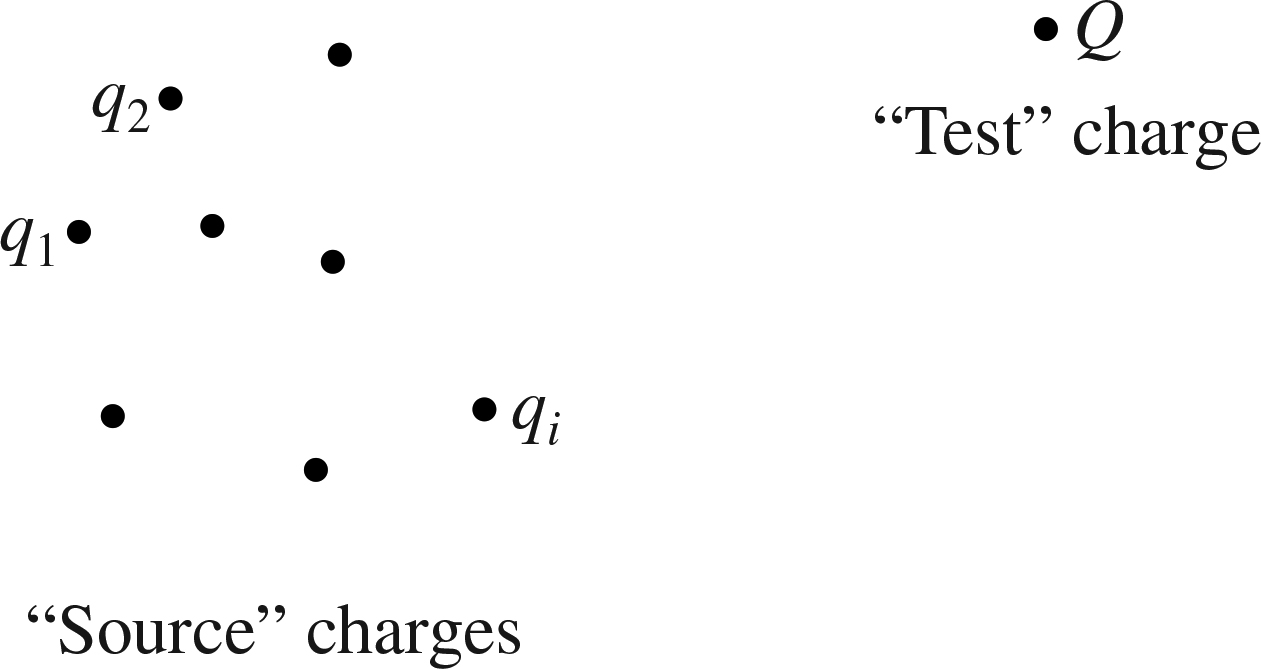
\includegraphics[width=5cm]{figures/2_1.jpg}
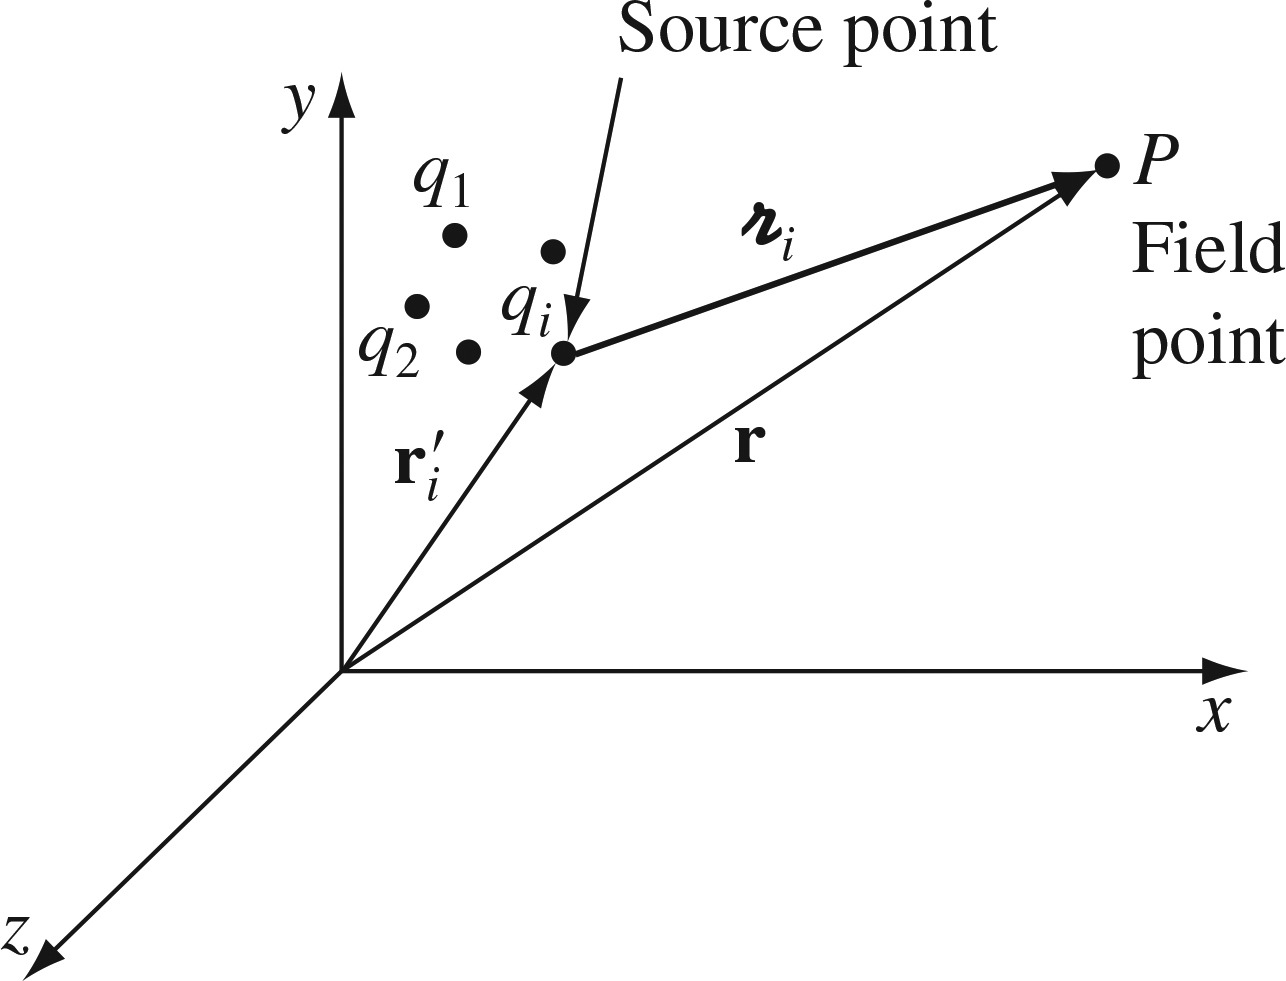
\includegraphics[width=5cm]{figures/2_3.jpg}
\caption{\label{fig:2_1} The basic problem of electrostatics. Note the definition of the separation vector, and the vectors to the field point and to all the source charges.}
\end{figure}
\end{frame}

\begin{frame}{Charge distributions, Superposition, and the Coulomb Force}
\begin{figure}
\centering
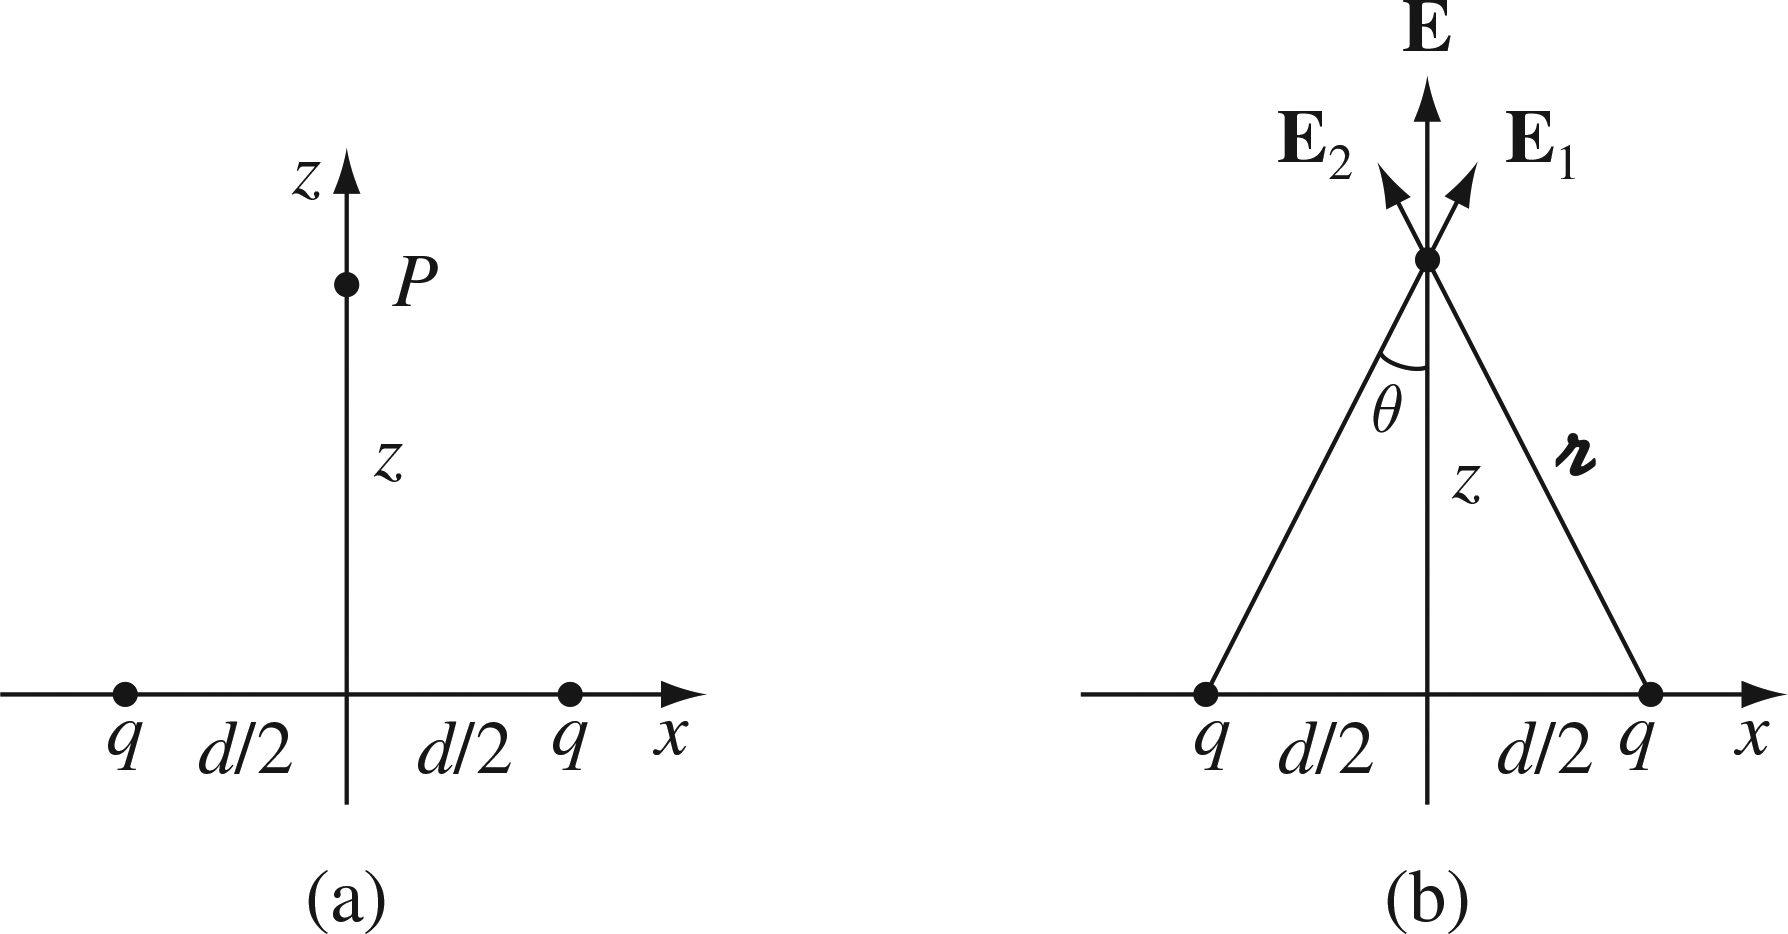
\includegraphics[width=10cm]{figures/2_4.jpg}
\caption{\label{fig:2_4} Begin with a dipole, and then a \textit{physical} dipole.}
\end{figure}
\end{frame}

\begin{frame}{Charge distributions, Superposition, and the Coulomb Force}
\begin{figure}
\centering
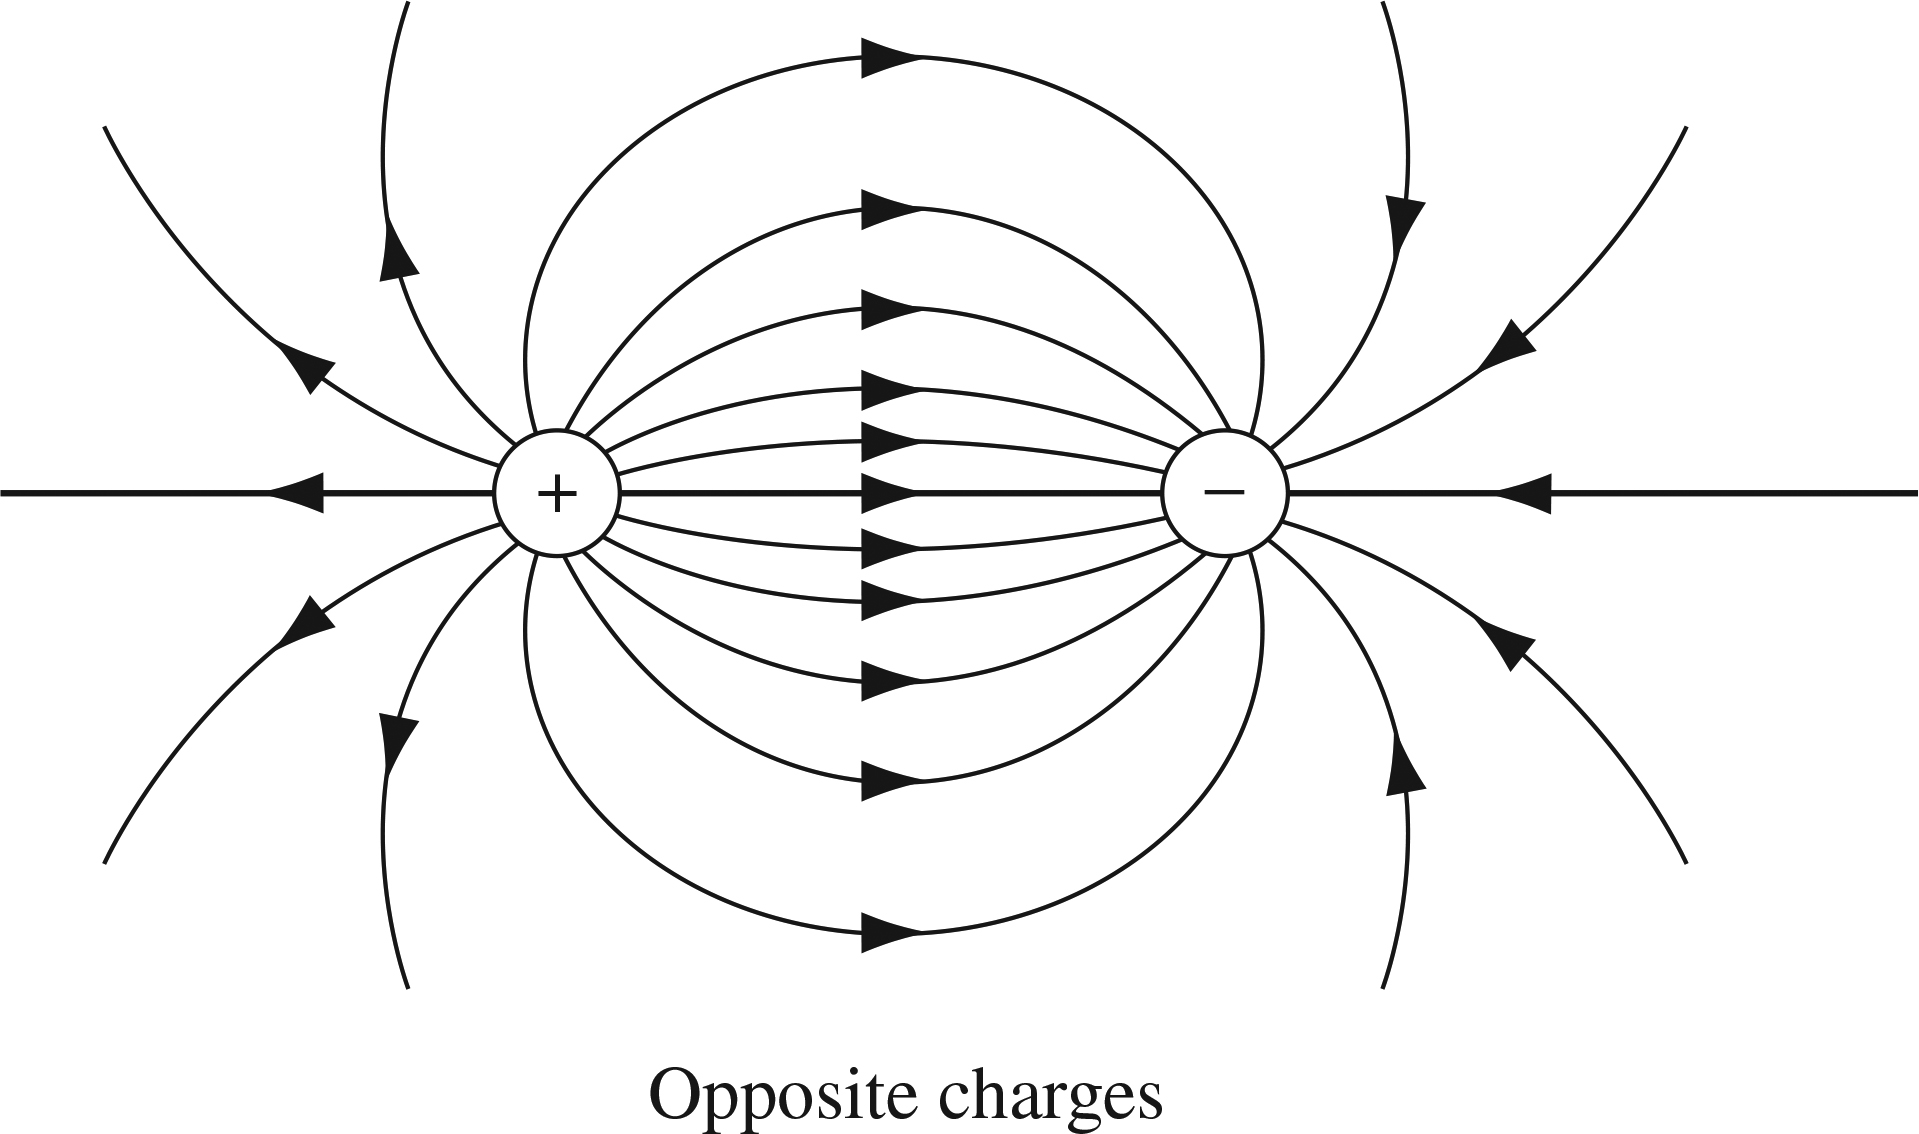
\includegraphics[width=10cm]{figures/2_13.jpg}
\caption{\label{fig:2_13} Field of a \textit{physical} dipole.}
\end{figure}
\end{frame}

\begin{frame}{Charge distributions, Superposition, and the Coulomb Force}
\begin{figure}
\centering
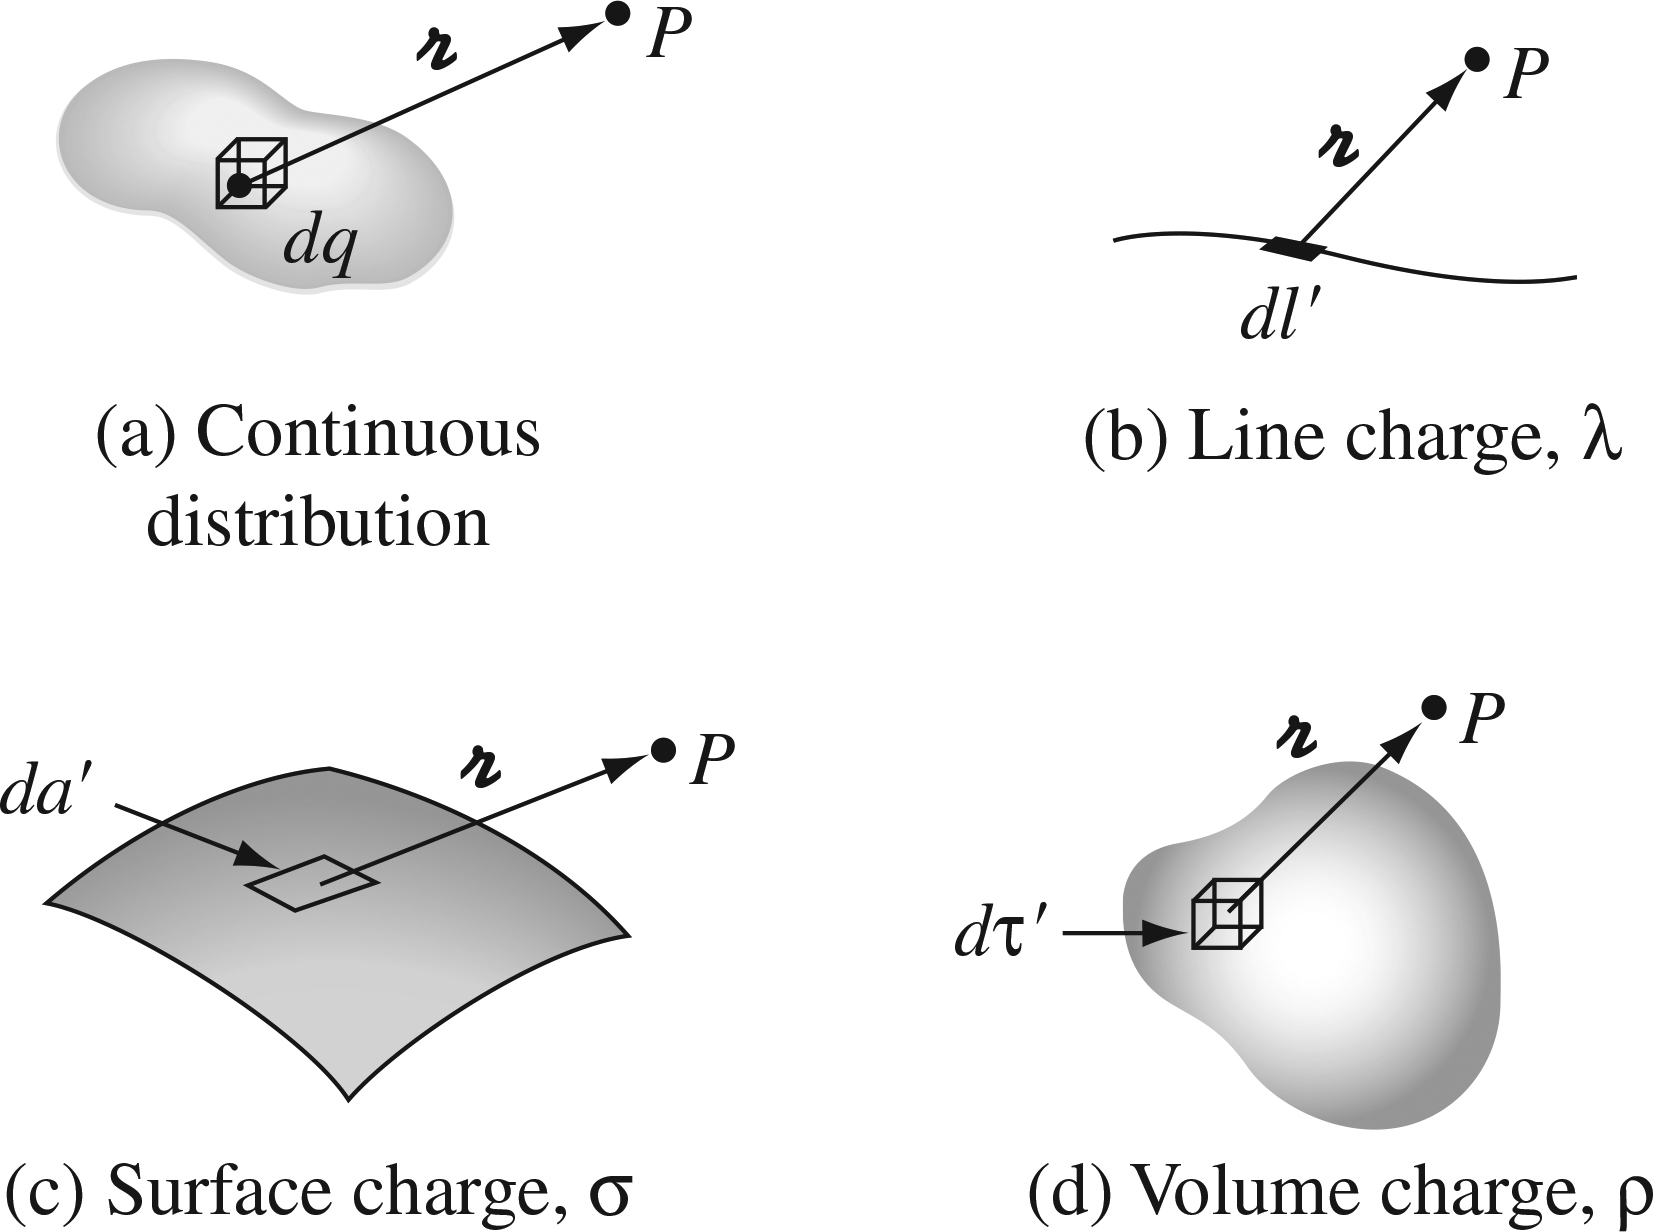
\includegraphics[width=8cm]{figures/2_5.jpg}
\caption{\label{fig:2_5} The continuous limit implies a variety of symmetries and geometries over which we integrate, rather than sum.}
\end{figure}
\end{frame}

\begin{frame}{Charge distributions, Superposition, and the Coulomb Force}
\begin{figure}
\centering
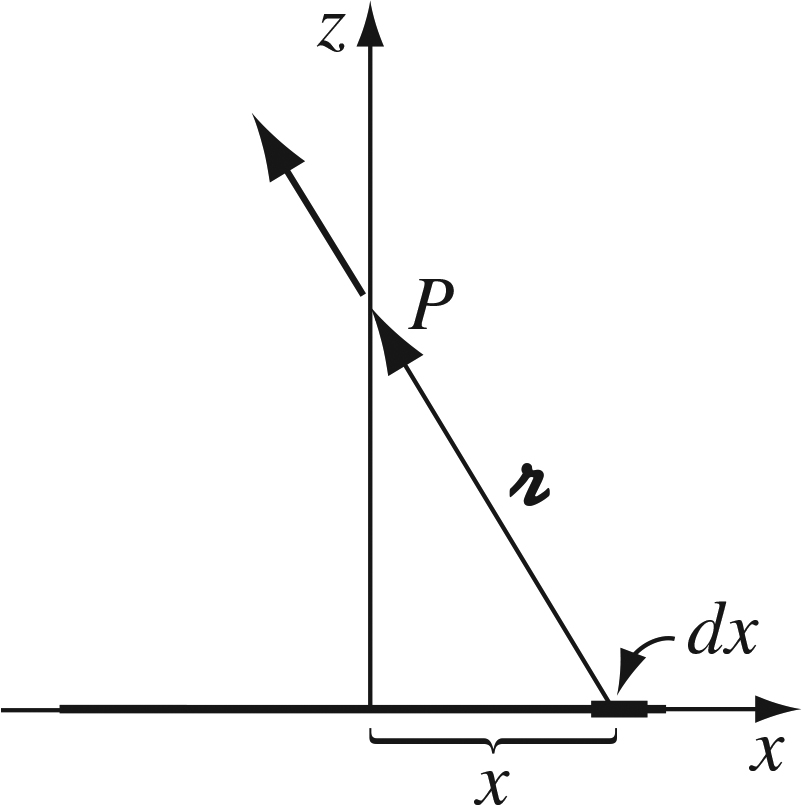
\includegraphics[width=6cm]{figures/2_6.jpg}
\caption{\label{fig:2_6} A coninuous line density of charge.  Integration yields the electric field.}
\end{figure}
\end{frame}

\begin{frame}{Charge distributions, Superposition, and the Coulomb Force}
\alert{Useful calculations:}
\begin{enumerate}
\item Continuous line charge, length $L$.
\item Continuous plane of charge, radius $R$.
\item Loop of charge, radius $R$, a distance $z$ above the center.
\end{enumerate}
Why are these interesting?  One example is that these shapes are used as \textit{antennas}.  Give some alternating current at the right voltage and impedance to a shape of metal, then you've got your antenna that radiates a certain way. \\ \vspace{1cm}
\textbf{Professor do these examples.}\footnote{Remember from PHYS180? Remember? Yeah...good times.}
\end{frame}

\section{A Note about the Far-Field}

\begin{frame}{The Far-Field}
\small
One way to express the \textbf{\alert{far-field}} approximation (compare to Fraunhofer and Fresnel limits in diffraction):
\begin{align}
\vec{r} &= \vec{r'} + \vec{\rcurs} \\
\vec{\rcurs} &= \vec{r} - \vec{r'} \\
\rcurs &= \sqrt{r^2 - 2 \vec{r} \cdot \vec{r'} + r'^2} \\
\rcurs &= r\sqrt{1 - 2 \vec{r} \cdot \vec{r'} r^{-2} + r'^2 r^{-2}} \\
\rcurs &\approx r\sqrt{1 - 2 \vec{r} \cdot \vec{r'} r^{-2}} \\
\rcurs &\approx r\left(1 - \vec{r} \cdot \vec{r'} r^{-2}\right) \\
\rcurs &\approx r\left(1 - \hat{r} \cdot \vec{r'} r^{-1}\right) \\
\rcurs &\approx r - \hat{r} \cdot \vec{r'}
\end{align}
\end{frame}

\begin{frame}{The Far-Field}
\small
\alert{\textbf{Repeat the charged loop calculation}}, but replace $\rcurs \approx r - \hat{r} \cdot \vec{r'}$ at the outset.  What happens? \\ \vspace{8cm}
\end{frame}

\section{The Divergence of $\vec{E}$-fields}

\begin{frame}{The Divergence of $\vec{E}$-fields}
\begin{figure}
\centering
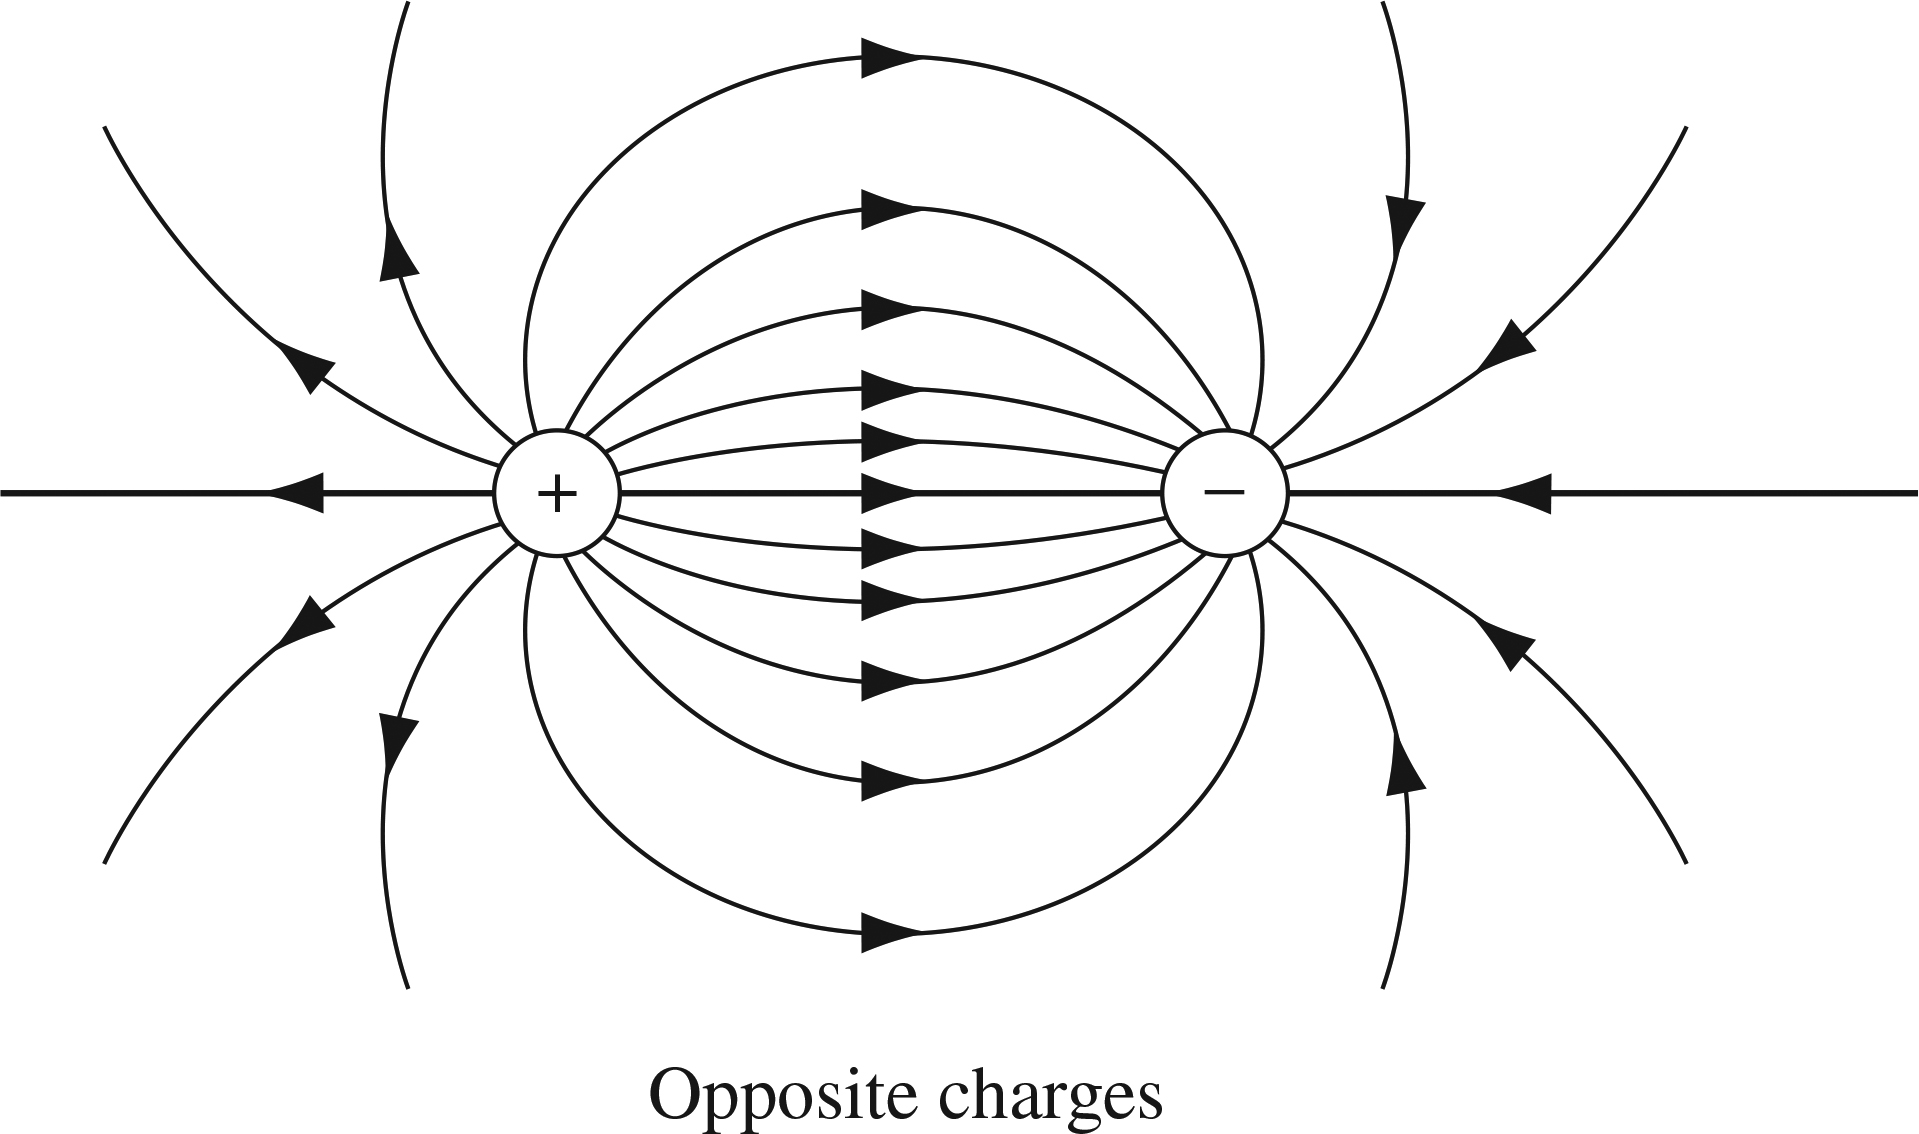
\includegraphics[width=5cm]{figures/2_13.jpg}
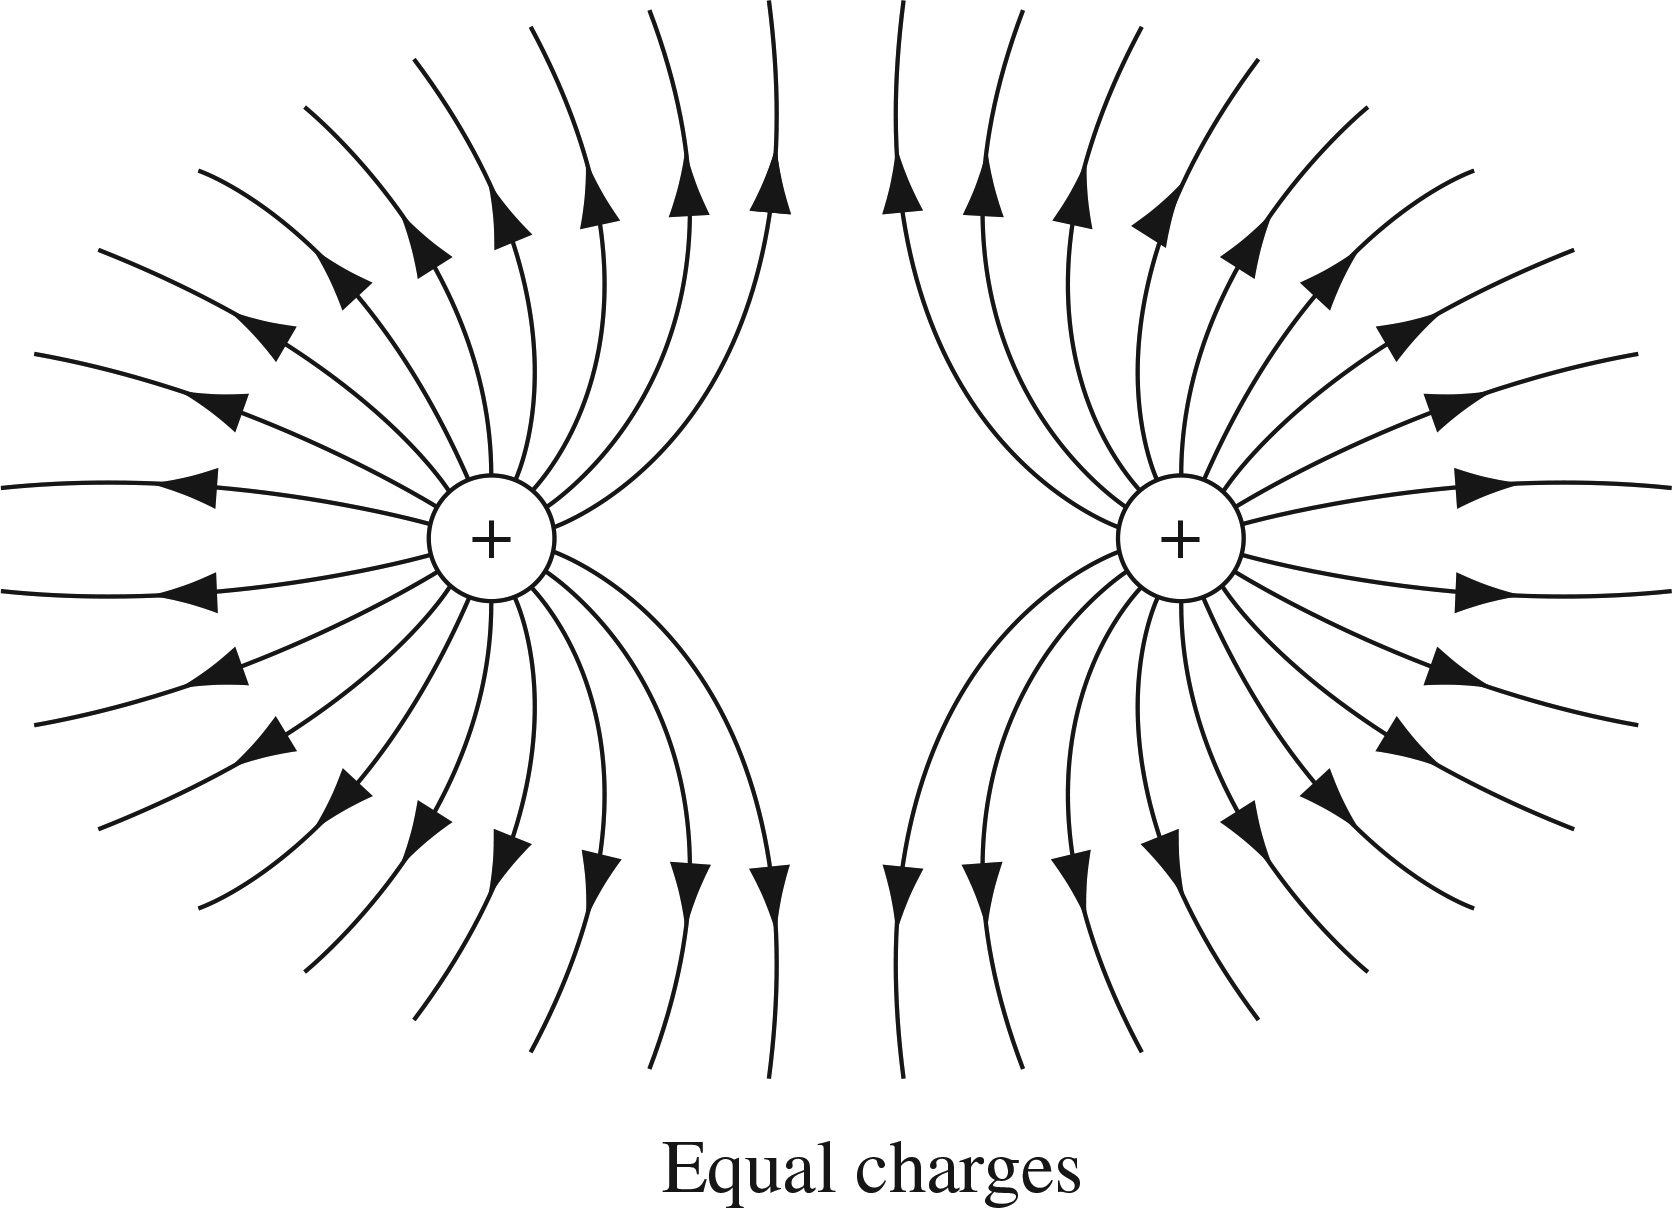
\includegraphics[width=4cm]{figures/2_14.jpg}
\caption{\label{fig:fieldLines} Field lines are an important theoretical concept.}
\end{figure}
\end{frame}

\begin{frame}{The Divergence of $\vec{E}$-fields}
\begin{figure}
\centering
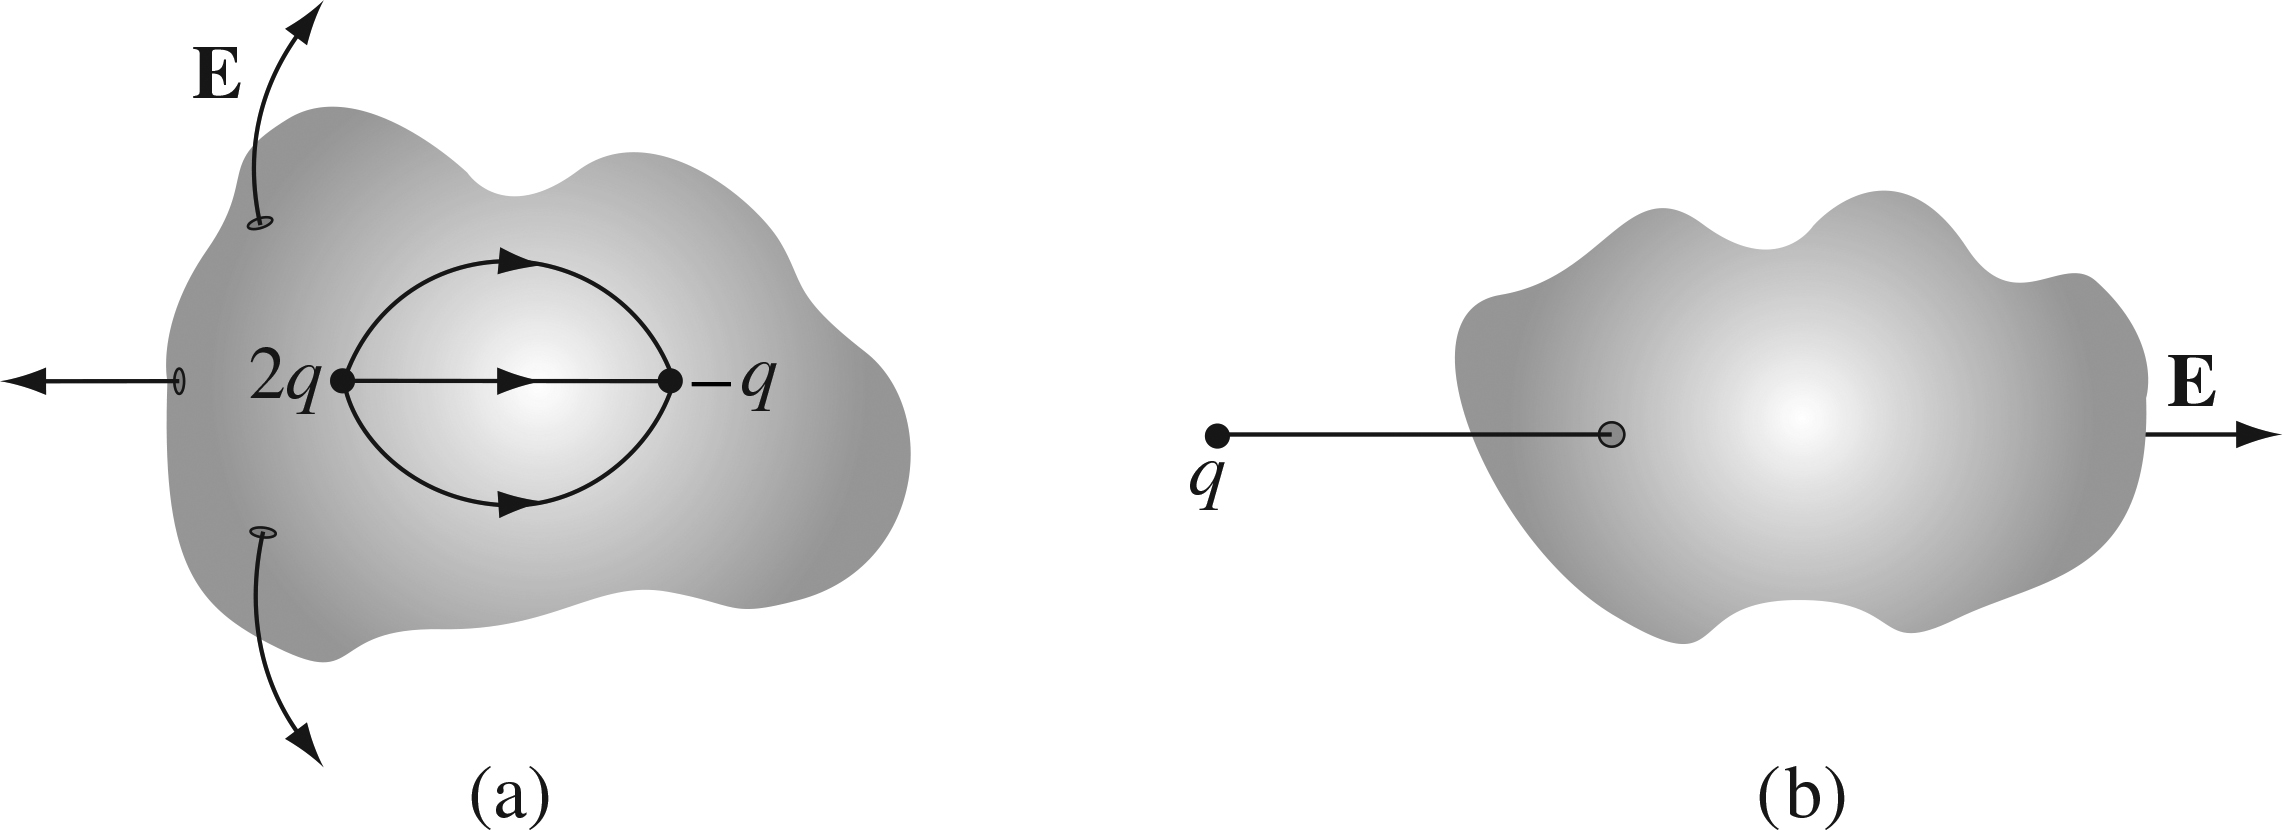
\includegraphics[width=10cm]{figures/2_16.jpg}
\caption{\label{fig:fieldLines2} The concept of a closed Gaussian surface.}
\end{figure}
\end{frame}

\begin{frame}{The Divergence of $\vec{E}$-fields}
\begin{equation}
\boxed{
\oint \vec{E_i} \cdot d\vec{a} = \frac{1}{4\pi \epsilon_0} \int_0^{\pi} \int_0^{2\pi} \frac{q_i\hat{r}}{r^2} \cdot r^2 \sin\theta d\theta d\phi \hat{r} = \frac{q_i}{\epsilon_0}
}
\end{equation}
\begin{align}
\vec{E} =& \sum_{i=1}^n \vec{E}_i \\
\oint \vec{E} \cdot d\vec{a} =& \sum_{i=1}^n \left(\oint \vec{E}_i \cdot d\vec{a}\right) \\
\oint \vec{E} \cdot d\vec{a} =& \sum_{i=1}^n \left( \frac{q_i}{\epsilon_0} \right) \\
\oint \vec{E} \cdot d\vec{a} =& \frac{Q_{tot}}{\epsilon_0}
\end{align}
\alert{Gauss' Law: the total flux is proportional to the contained charge.}
\end{frame}

\begin{frame}{The Divergence of $\vec{E}$-fields}
The divergence theorem:
\begin{equation}
\oint_{\mathcal{S}} \vec{E} \cdot d\vec{a} = \int_{\mathcal{V}} (\nabla \cdot \vec{E}) d\tau
\end{equation}
Remark that the total charge is the integral over the 3D charge density:
\begin{equation}
\frac{Q_{tot}}{\epsilon_0} = \frac{1}{\epsilon_0}\int_{\mathcal{V}} \rho d\tau
\end{equation}
This implies
\begin{equation}
\oint_{\mathcal{S}} \vec{E} \cdot d\vec{a} = \int_{\mathcal{V}} (\nabla \cdot \vec{E}) d\tau = \frac{1}{\epsilon_0}\int_{\mathcal{V}} \rho d\tau
\end{equation}
Looking at the last two expressions:
\begin{equation}
\boxed{
\nabla \cdot \vec{E} = \frac{\rho}{\epsilon_0}
}
\end{equation}
\end{frame}

\begin{frame}{The Divergence of $\vec{E}$-fields}
\textit{Differential form} of Gauss' Law:
\begin{equation}
\boxed{
\nabla \cdot \vec{E} = \frac{\rho}{\epsilon_0}
}
\end{equation}
Consider a different argument:
\begin{align}
\vec{E} =& \frac{1}{4\pi\epsilon_0} \int \frac{\hrcurs}{\rcurs^2} \rho(\vec{r}') d\tau' \label{eq:E} \\
\nabla \cdot \vec{E} =& \frac{1}{4\pi\epsilon_0} \int \nabla \cdot \left(\frac{\hat{\hrcurs}}{\rcurs^2} \right)\rho(\vec{r}') d\tau' \\
\nabla \cdot \vec{E} =& \frac{1}{4\pi\epsilon_0} \int 4\pi \delta^3(\brcurs)\rho(\vec{r}') d\tau' \\
\nabla \cdot \vec{E} =& \frac{4\pi}{4\pi\epsilon_0} \int \delta^3(\vec{r} - \vec{r}')\rho(\vec{r}') d\tau' \\
\nabla \cdot \vec{E} =& \rho(\vec{r})/\epsilon_0
\end{align}
\end{frame}

\begin{frame}{The Divergence of $\vec{E}$-fields}
\textbf{\alert{Symmetry in the Application of Gauss' Law}}: \\
If the E-field and the area element are \textit{always} orthogonal,
\begin{align}
\oint \vec{E} \cdot d\vec{a} =& \frac{Q_{tot}}{\epsilon_0} \\
|\vec{E}| A =& \frac{Q_{tot}}{\epsilon_0} \\
\vec{E} =& \frac{Q_{tot}}{\epsilon_0 A} \hat{n}
\end{align}
This trick can be used even when the charge distribution is not uniform, but \textit{does exhibit} symmetry.
\end{frame}

\begin{frame}{The Divergence of $\vec{E}$-fields}
\begin{figure}
\centering
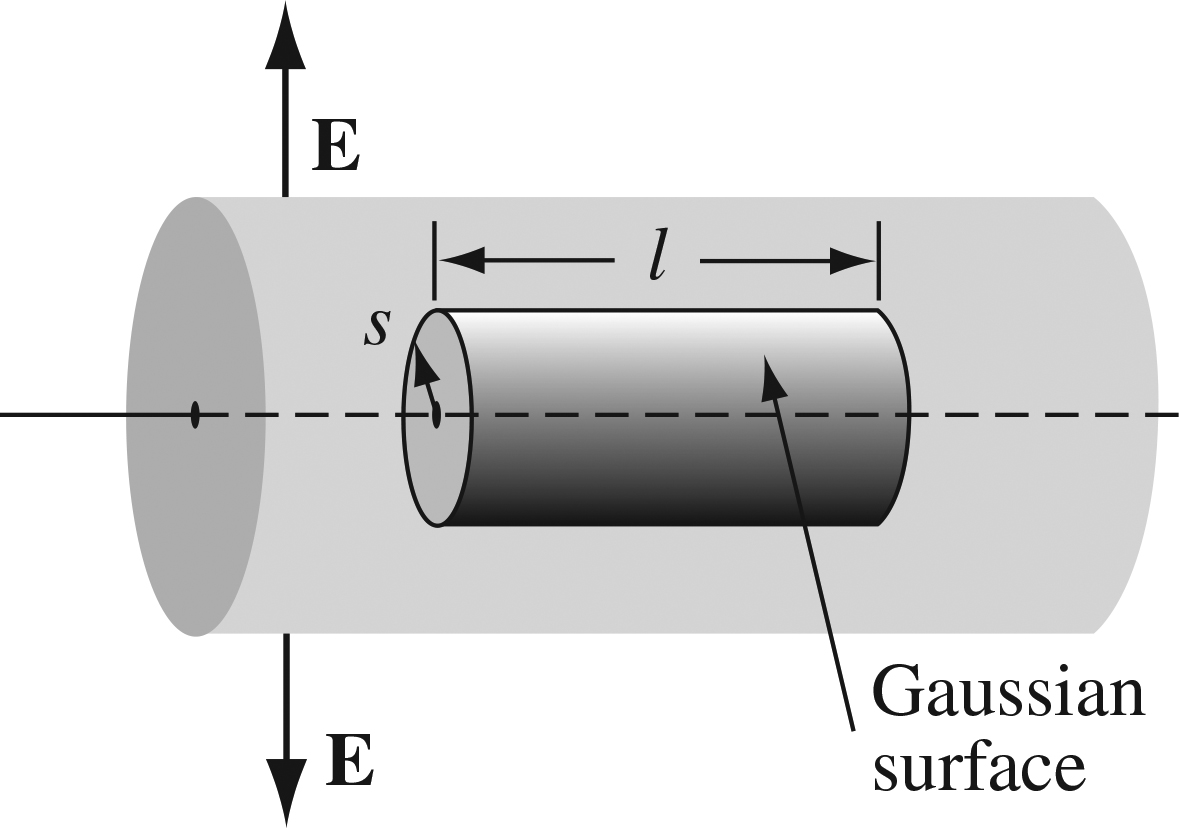
\includegraphics[width=7cm]{figures/2_21.jpg}
\caption{\label{fig:cyl} Use cylindrical symmetry to apply Gauss' Law.  The charge distribution function is $\rho(s) = ks$.  Obtain the field (a) \textit{inside} the object, then (b) outside the object.}
\end{figure}
\end{frame}

\begin{frame}{The Divergence of $\vec{E}$-fields}
\begin{figure}
\centering
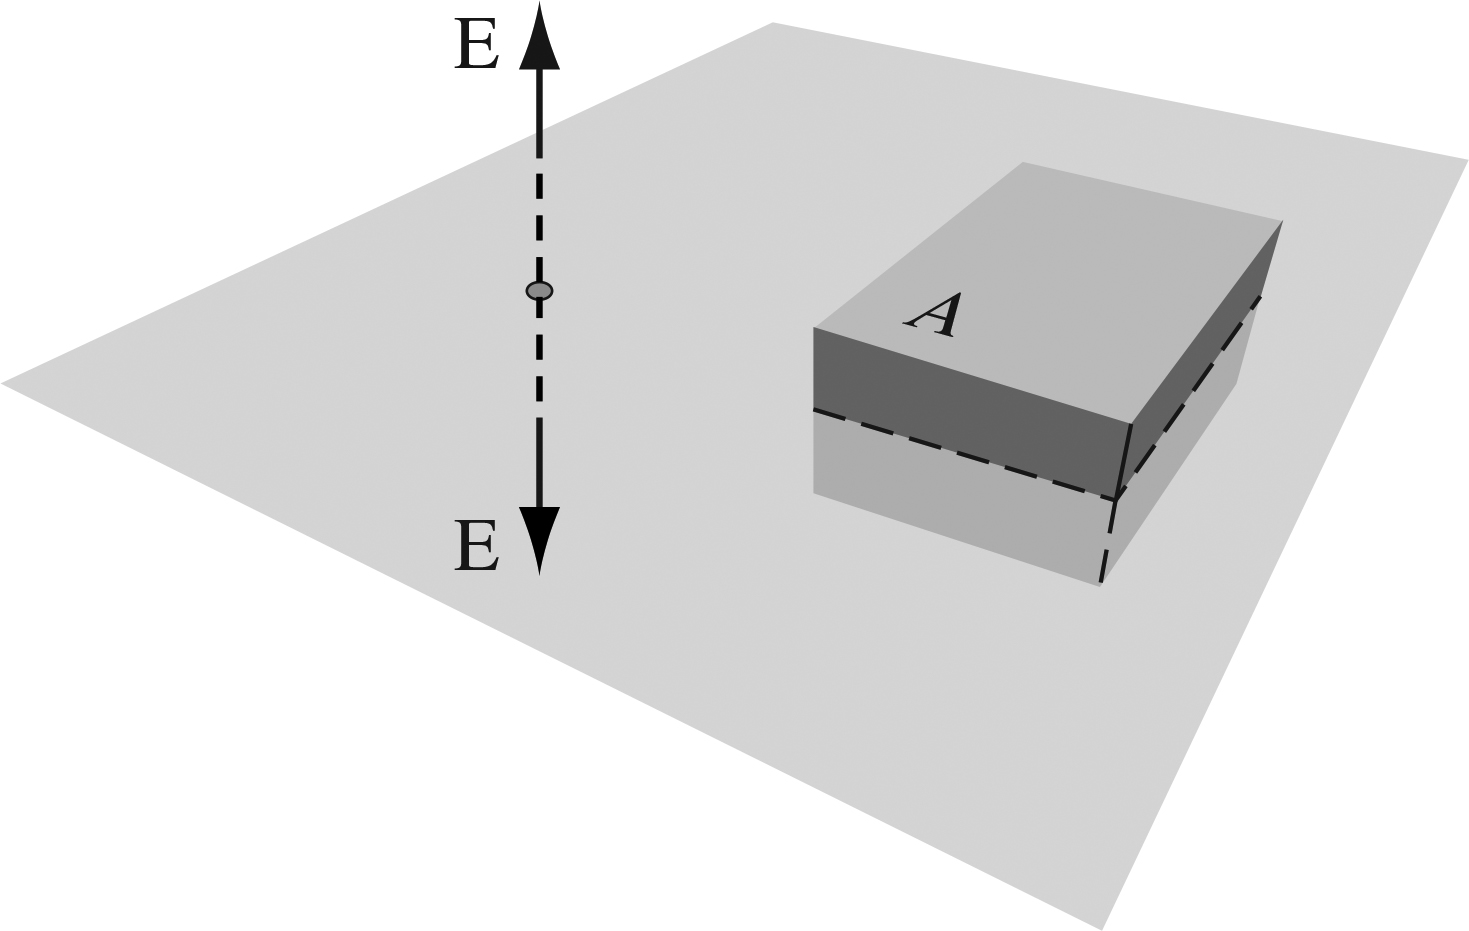
\includegraphics[width=7cm]{figures/2_22.jpg}
\caption{\label{fig:cyl2} Use Cartesian symmetry to apply Gauss' Law.  The charge distribution function is $\rho(x,y) = +\sigma$.  Obtain the field above (or below) the charged plane.}
\end{figure}
\end{frame}

\begin{frame}{The Divergence of $\vec{E}$-fields}
\begin{figure}
\centering
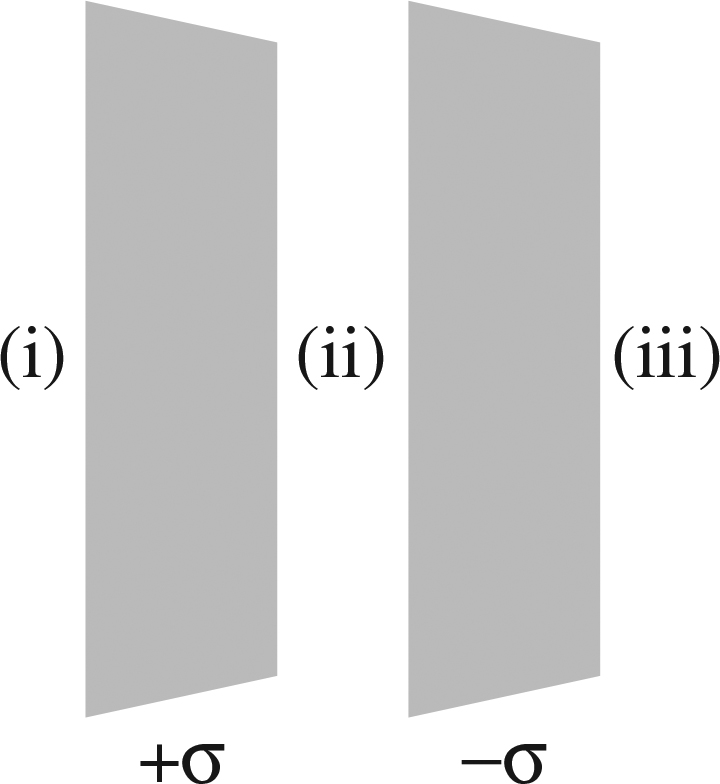
\includegraphics[width=5cm]{figures/2_23.jpg}
\caption{\label{fig:cyl3} Combinations of ``Gaussian charged objects.''  What about the field between two line charges?}
\end{figure}
\end{frame}

\section{The Curl of $\vec{E}$-fields}

\begin{frame}{The Curl of $\vec{E}$-fields}
The $\vec{E}$-field of a point charge at the origin ($\vec{r}' = 0$), and the line element in spherical coordinates:
\begin{align}
\vec{E} &= \frac{1}{4\pi\epsilon_0} \frac{q}{r^2} \hat{r} \\
d\vec{l} &= dr\hat{r} + rd\theta \hat{\theta} + r\sin\theta d\phi \hat{\phi} \\
\vec{E} \cdot d\vec{l} &= \frac{1}{4\pi\epsilon_0} \frac{q}{r^2} dr \\
\int_{\vec{a}}^{\vec{b}} \vec{E} \cdot d\vec{l} &= \frac{q}{4\pi\epsilon_0} \left(\frac{1}{r_a} - \frac{1}{r_b} \right) \\
\oint \vec{E} \cdot d\vec{l} &=  0 ~~ (\vec{a} = \vec{b}) \\
\nabla \times \vec{E} &= 0
\end{align}
Any combination of point charges will also lead to zero curl.  Why?  Superposition.
\end{frame}

\begin{frame}{The Curl of $\vec{E}$-fields}
\small
Define a function, then, that encapsulates \textit{path-independence}:
\begin{equation}
V(\vec{r}) = -\int_{\mathcal{O}}^{\vec{r}} \vec{E} \cdot d\vec{l}
\end{equation}
\begin{itemize}
\item $\mathcal{O}$ is a reference point, naturally taken to be $\infty$ (far from origin)
\item $V(\vec{b}) - V(\vec{a}) = -\int_{\vec{a}}^{\vec{b}} \vec{E} \cdot d\vec{l}$
\item $0 = V(\vec{a}) - V(\vec{a}) = -\oint \vec{E} \cdot d\vec{l} = 0$
\end{itemize}
Fundamental theorem for gradients:
\begin{align}
V(\vec{b}) - V(\vec{a}) &= \int_{\vec{a}}^{\vec{b}} \nabla V \cdot d\vec{l} = -\int_{\vec{a}}^{\vec{b}} \vec{E} \cdot d\vec{l} \\
\vec{E} &= -\nabla V
\end{align}
\end{frame}

\begin{frame}{The Curl of $\vec{E}$-fields}
\small
Path independence:
\begin{figure}
\centering
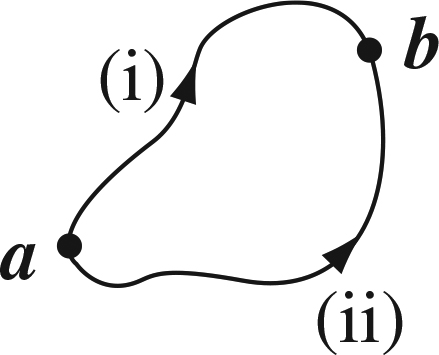
\includegraphics[width=4.5cm]{figures/2_30.jpg}
\caption{\label{fig:path1} If the line integral was not path-independent, then path i minus path ii would not be zero.  Path i and ii form a closed line integral.}
\end{figure}
\end{frame}

\begin{frame}{The Curl of $\vec{E}$-fields}
\small
Two more ideas:
\begin{align}
\vec{E} &= -\nabla V \\
\nabla \cdot \vec{E} &= - \nabla^2 V \\
\nabla^2 V &= -\frac{\rho}{\epsilon_0} \label{eq:pois}
\end{align}
Equation \ref{eq:pois} is known as the \textit{Poisson Equation}.  If $\rho = 0$ in some region:
\begin{equation}
\boxed{
\nabla^2 V = 0 \label{eq:laplace}
}
\end{equation}
Equation \ref{eq:laplace} is known as the Laplacian of the potential or Laplace's Equation.  Solving it is the subject of Ch. 3.
\end{frame}

\begin{frame}{The Curl of $\vec{E}$-fields}
Show that the potential of a point charge $q$ at the origin is
\begin{equation}
V(r) = \frac{1}{4\pi\epsilon_0} \frac{q}{r}
\end{equation}
Indeed, collections of point charges lead to 
\begin{equation}
V(r) = \frac{1}{4\pi\epsilon_0} \sum_i \frac{q_i}{\rcurs_i}
\end{equation}
A collection of \textit{many} point charges smoothed into a continuous distribution leads to
\begin{equation}
V(r) = \frac{1}{4\pi\epsilon_0} \int \frac{dq}{\rcurs} = \frac{1}{4\pi\epsilon_0} \int \frac{\rho' d\tau'}{\rcurs}
\end{equation}
\end{frame}

\begin{frame}{The Curl of $\vec{E}$-fields}
\begin{equation}
V(r) = \frac{1}{4\pi\epsilon_0} \int \frac{\rho' d\tau'}{\rcurs}
\end{equation}
(a) Derive the potential due to a line charge of length $L$, directly above the center of the line. (b) Take the gradient in cylindrical coordinates to obtain $\vec{E}$. \\ \vspace{6cm}
\end{frame}

\section{Brief Remark about Boundary Conditions}

\begin{frame}{Boundary Conditions}
\begin{figure}
\centering
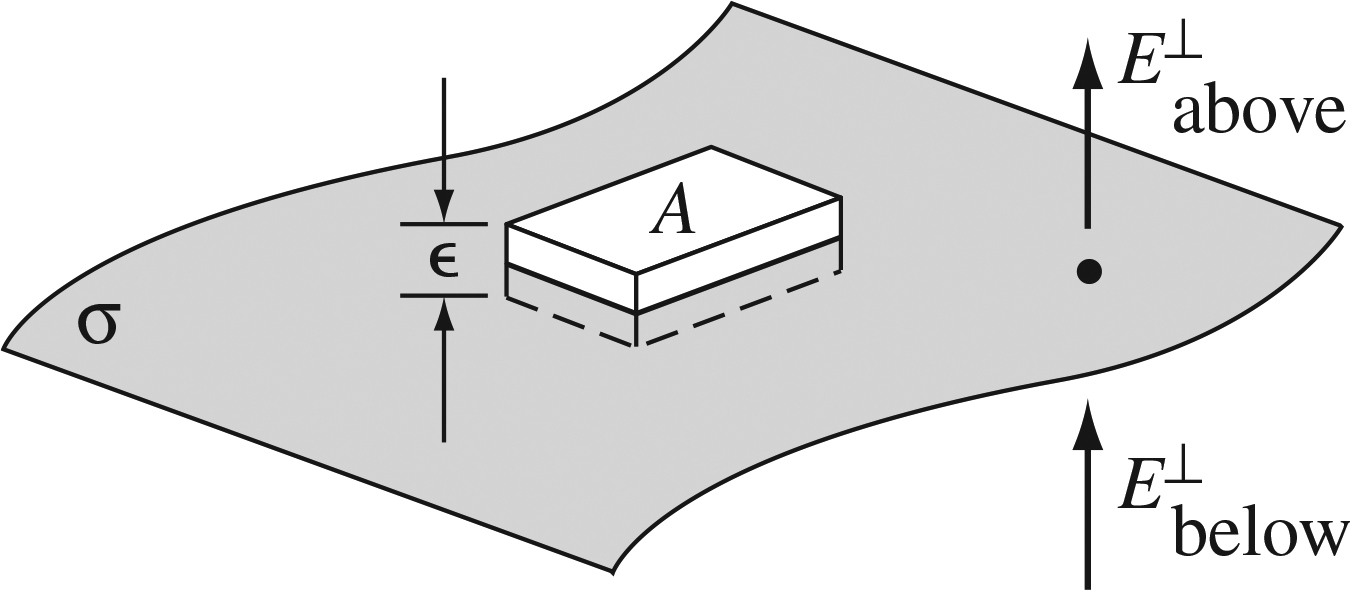
\includegraphics[width=4cm]{figures/2_36.jpg}
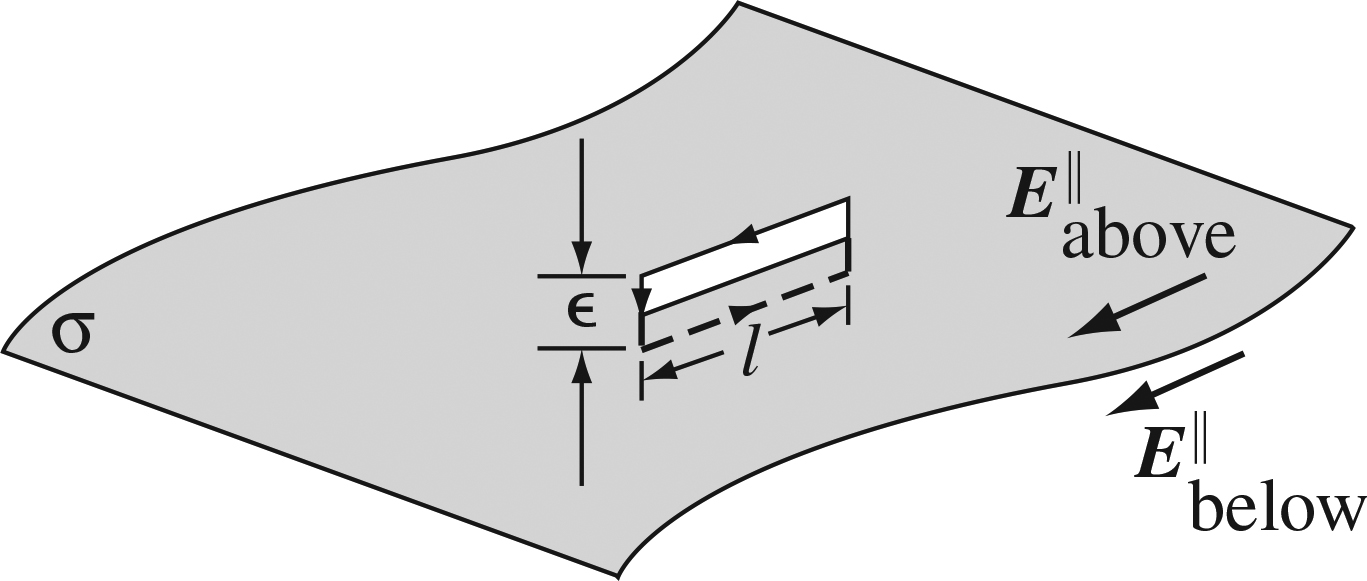
\includegraphics[width=4cm]{figures/2_37.jpg}
\caption{\label{fig:bound} (Left) By Gauss' Law, we may find the discontinuity in the orthogonal E-field component. (Right) Via a closed-loop line integral, we may find that the parallel component of the E-field is continuous.}
\end{figure}
\begin{align}
\left(\nabla V_{top} - \nabla V_{bottom}\right) \cdot \hat{n} &= -\frac{\sigma}{\epsilon_0} \\
\left(\nabla V_{top} - \nabla V_{bottom}\right) \cdot \hat{s} &= 0
\end{align}
\end{frame}

\begin{frame}{Boundary Conditions}
Which of the following functions has a discontinuity \textit{in the derivative} but not the function itself, at $x = 0$?
\begin{itemize}
\item A: $\tan(x)$
\item B: $|x| = abs(x)$
\item C: $\sqrt{x}$
\item D: $\theta(x)$ (Heaviside step-function)
\end{itemize}
\end{frame}

\begin{frame}{Boundary Conditions}
\alert{Consult your notes regarding the charge distribution with spherical symmetry}.
\begin{itemize}
\item What was the formula for the electric field as a function of $r$, when $r<R$?
\item What is the correct formula for the electric field as a function of $r$, when $r\geq R$? (\textit{Think of Gauss' Law}).
\item What is the voltage just outside the radius $R$?
\item What is the voltage just inside the radius $R$?
\end{itemize}
\end{frame}

\section{Energy and Work}

\begin{frame}{Energy and Work}
The work required to assemble point charges by bring each in from infinity is 
\begin{equation}
W = \frac{1}{2}\sum_{i=1}^n q_i \left( \sum_{j\neq i}^{n} \frac{1}{4\pi\epsilon_0} \frac{q_j}{\rcurs_{ij}}\right)
\end{equation}
The parentheses contains the potential due to all charges except $q_i$:
\begin{equation}
W = \frac{1}{2}\sum_{i=1}^n q_i V(\vec{\rcurs}_i)
\end{equation}
Note that it doesn't matter when charge $q_i$ arrived; we have to pay for the energy used to keep $q_i$ there as everyone else arrives as well.
\end{frame}

\begin{frame}{Energy and Work}
Continuous limit:
\begin{equation}
\boxed{
W = \frac{1}{2} \int \rho(r') V(r') d\tau'
}
\end{equation}
This result can be re-written:
\begin{equation}
W = \frac{\epsilon_0}{2} \left\lbrace -\int \vec{E} \cdot (\nabla V) d\tau + \oint V \vec{E} \cdot d\vec{a} \right \rbrace
\end{equation}
Like any integration by parts, there is an integral term and a surface term (the second term).  Use $-\vec{E} = \nabla V$, and expand the Gaussian surface so far that all contributions from the second term vanish:
\begin{equation}
W = \frac{\epsilon_0}{2} \int E^2 d\tau
\end{equation}
\end{frame}

\begin{frame}{Energy and Work}
Since we do not specify the shape of the volume, we can speak about the \textit{energy per unit volume}:
\begin{equation}
\boxed{
u_E = \frac{\epsilon_0}{2}E^2
}
\end{equation}
\begin{itemize}
\item E-fields contain energy
\item This equation is valid even if E-field values vary in space (of course)
\item Consider the simple example of a capacitor ...
\end{itemize}
\end{frame}

\begin{frame}{Energy and Work}
Start with the E-field inside a parallel-plate capacitor:
\begin{align}
E &= \frac{\sigma}{\epsilon_0} \\
u_E &= \frac{1}{2\epsilon_0}\sigma^2 \\
\mathcal{E} &= \frac{Ad}{2\epsilon_0}\sigma^2 \\
\sigma &= \frac{Q}{A} \\
C &= \frac{\epsilon_0 A}{d} \\
\mathcal{E} &= \frac{1}{2} \frac{Q^2}{C} = \frac{1}{2}C V^2 = U
\end{align}
Energy conservation.
\end{frame}

\section{Conclusion}

\begin{frame}{Week 2 Summary}
\begin{enumerate}
\item Homework discussions
\begin{itemize}
\item Proofs!  Glorious proofs.
\item Exercises with \textit{checking} fundamental theorems
\end{itemize}
\item Electrostatics and Coulomb forces
\begin{itemize}
\item Charge distributions, superposition, and the Coulomb force
\item A note about the \textit{far-field}
\item Setting up integrals, taking limits, checking units
\item The divergence of electric fields
\item The curl of electric fields
\end{itemize}
\item Electric Potential
\begin{itemize}
\item Definitions, fundamental theorem for gradients
\item Reference points
\item Laplace equation ...
\end{itemize}
\item Work, energy, and conductors
\end{enumerate}
\end{frame}

\end{document}
